\begin{center}
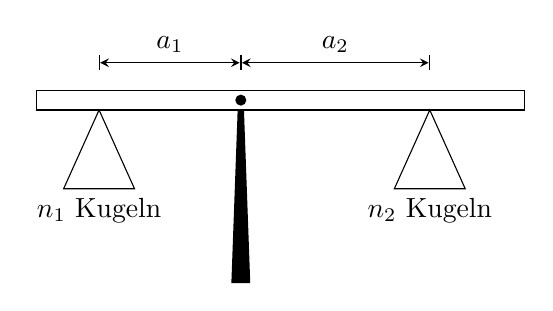
\begin{tikzpicture}[>=stealth]
 \fill (-0.12,-2.2) -- (0.12,-2.2) -- (0.04,0) -- (-0.04,0) -- cycle;
 \draw[fill=white] (-2.6,0) rectangle (3.6,0.25);
 \fill (0,0.125) circle (0.07);
 \draw (-1.8,0) -- (-2.25,-1.0) -- (-1.35,-1.0) -- cycle;
 \draw (2.4,0) -- (1.95,-1.0) -- (2.85,-1.0) -- cycle;
 \draw[|<->|] (-1.8,0.6) -- (0,0.6) node[midway, above] {$a_1$};
 \draw[|<->|] (0,0.6) -- (2.4,0.6) node[midway, above] {$a_2$};
 \node[below] at (-1.8,-1.0) {$n_1$ Kugeln};
 \node[below] at (2.4,-1.0) {$n_2$ Kugeln};
\end{tikzpicture}
\end{center}

Wir nehmen an, dass die leere Waage im Gleichgewicht ist. Jede Kugel habe die Gewichtskraft $F$. Mit $n_1$ Kugeln im Abstand $a_1 = \aWaO$ und $n_2$ Kugeln im Abstand $a_2 = \bWaO$ verlangt das Hebelgesetz
\begin{align}
 n_1 F\cdot a_1 &= n_2 F\cdot a_2 \quad\Rightarrow\quad \frac{n_1}{n_2} = \frac{a_2}{a_1}
\end{align}
Zusammen mit $n_1 + n_2 = N$ folgt
\begin{align}
 n_1 &= \nWaF = \frac{\bWa}{\aWa+\bWa}\cdot\NWa = \result{\nWaI} \\
 n_2 &= \nWbF = \frac{\aWa}{\aWa+\bWa}\cdot\NWa = \result{\nWbI}
\end{align}
Auf die Schale näher an der Drehachse gehören also \nWaI\ Kugeln, auf die andere \nWbI.
